\documentclass[12pt,a4paper,twoside]{article}
    \special{papersize=210mm,297mm}
    %\usepackage{fullpage}
    \usepackage[a4paper,includeheadfoot,margin=2.54cm]{geometry}

    \usepackage{hyperref}

    \usepackage[utf8]{inputenc}
    \usepackage{graphicx}
    \usepackage[danish]{babel}

    \usepackage[familydefault,regular]{Chivo}
    \usepackage[T1]{fontenc}

    \usepackage{lastpage}
    \usepackage{fancyhdr}
    \pagestyle{fancy} 
    \fancyhf{}
    \fancyhead[LE,RO]{Et kig på IBI i privaten}
    \fancyhead[RE,LO]{\rightmark}
    \fancyfoot[CE,CO]{Michael Torp Kaalund, Hold: elsp4d18}
    \fancyfoot[LE,RO]{Side \thepage \hspace{1pt} af \pageref{LastPage}}
    \renewcommand{\headrulewidth}{1.5pt}
    \renewcommand{\footrulewidth}{1.5pt}

    %\usepackage{showframe}
 
    \title{Et kig på IBI i privaten}
    
    \author{Michael Torp Kaalund \thanks{Mange tak til min læreplads Intego A/S}}
    
    \begin{document}

    \begin{titlepage}
    \centering
    {\usefont{T1}{pag}{m}{b}\LARGE Den jydske håndværkerskole i Hadsten \par}
    \vspace{1cm}
    {\usefont{T1}{fvs}{m}{b}\Large Svendeprøve som elektriker \par}
    \vspace{1.5cm}
    {\huge\bfseries Et kig på IBI i privatboligen \par}
    \vspace{10cm}
    {\usefont{T1}{qzc}{m}{it} Michael Torp Kaalund, Intego A/S Randers afd. \par}
    {\usefont{T1}{qzc}{m}{it} Hold: elsp4d18 \par}
    \vfill
    {\bfseries \today\par}
\end{titlepage}


    \begin{abstract}
        TODO: Skrive omkring hvad projektet går ud på.
    \end{abstract}

    \newpage

    \tableofcontents

    \newpage

    \section{Fonts}
    Her har jeg skrevet hvilke fonte

    \appendix

    \newpage
\subsection{Siemens LOGO!}

%\newpage
\subsubsection{Siemens LOGO! manual, side 41}
%\cite{logo_sm} Manual
\label{man:logo_side_41}
\includegraphics[scale=0.72]{appendix/siemens/logo_system_manual_41.pdf}

\subsubsection{Siemens LOGO! manual, side 42}
%\cite{logo_sm} Manual
\label{man:logo_side_42}
\includegraphics[scale=0.72]{appendix/siemens/logo_system_manual_42.pdf}

\subsubsection{Tavledokumentation}
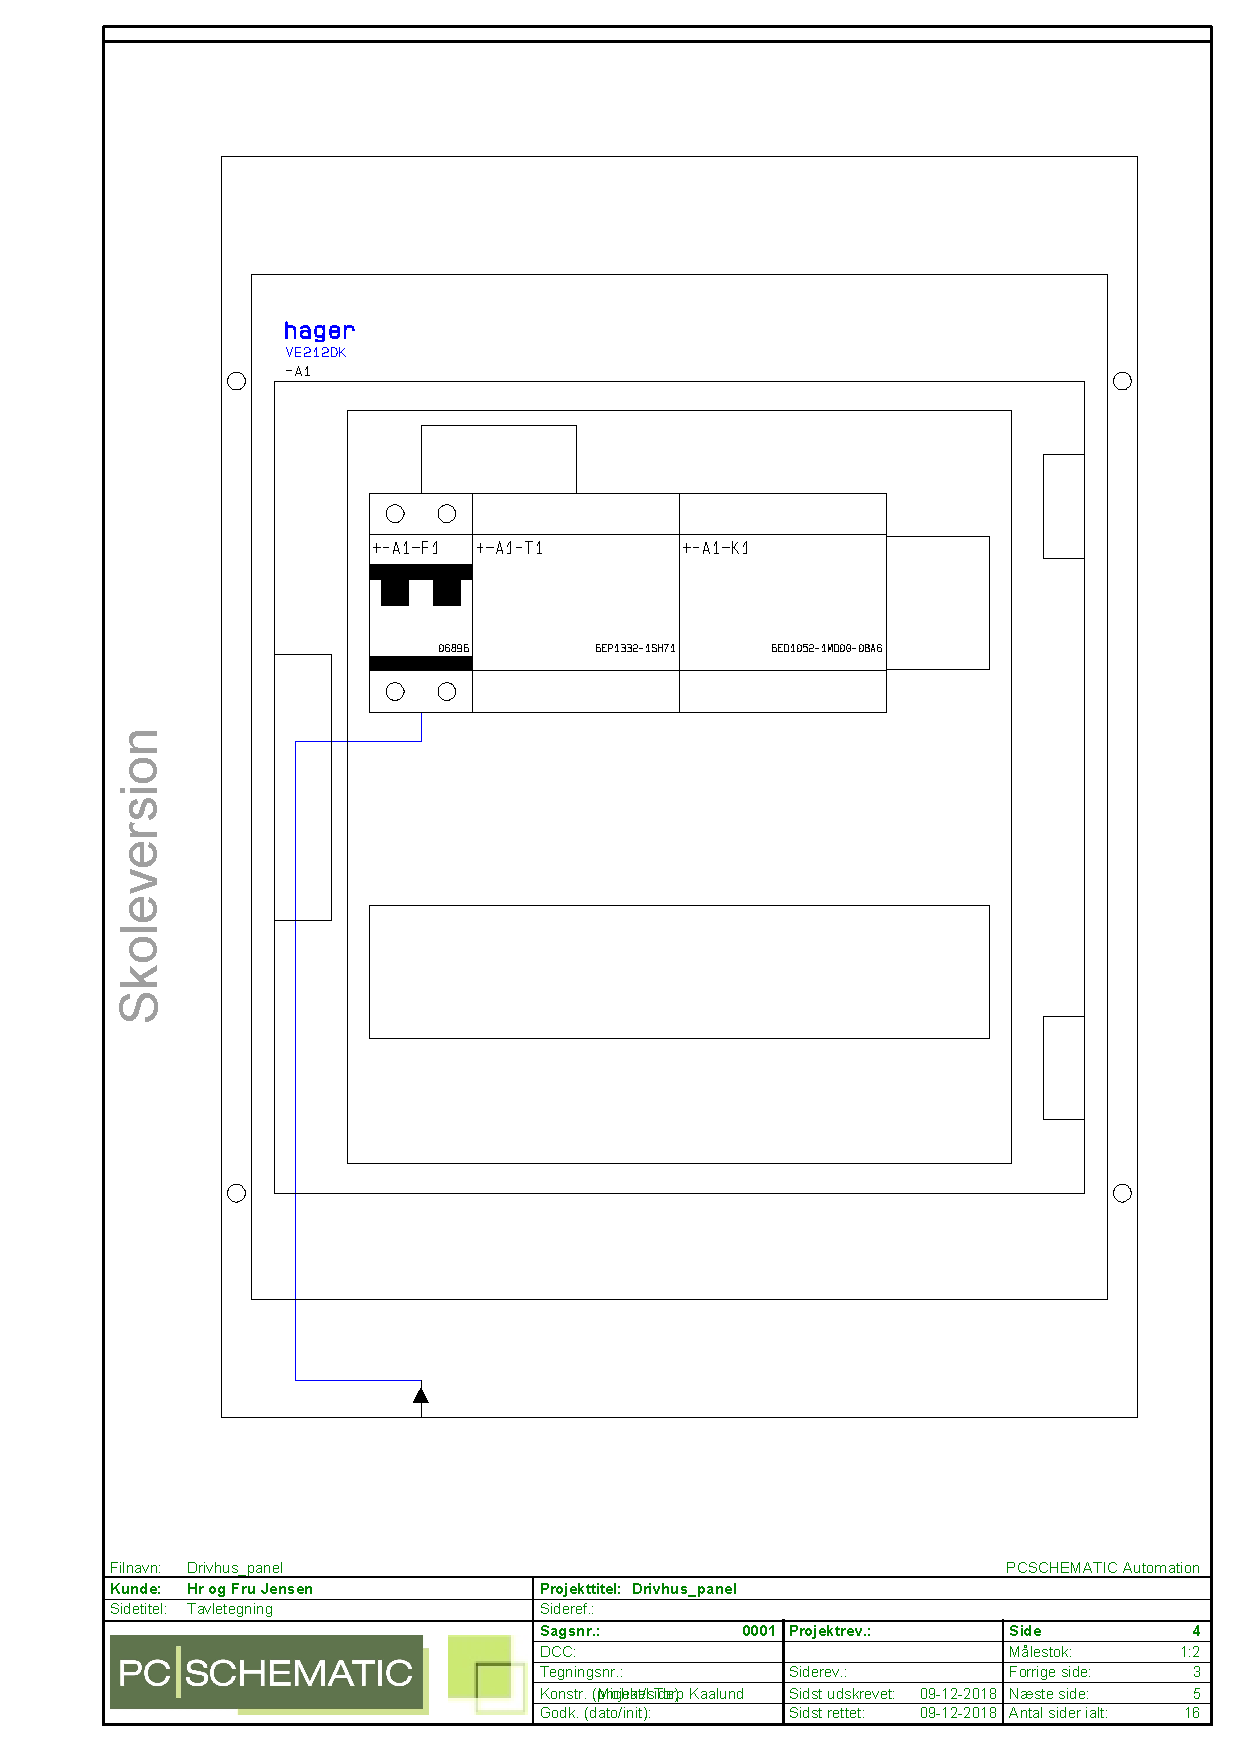
\includegraphics[scale=0.72]{appendix/Drivhus_panel_5.pdf}
\newpage
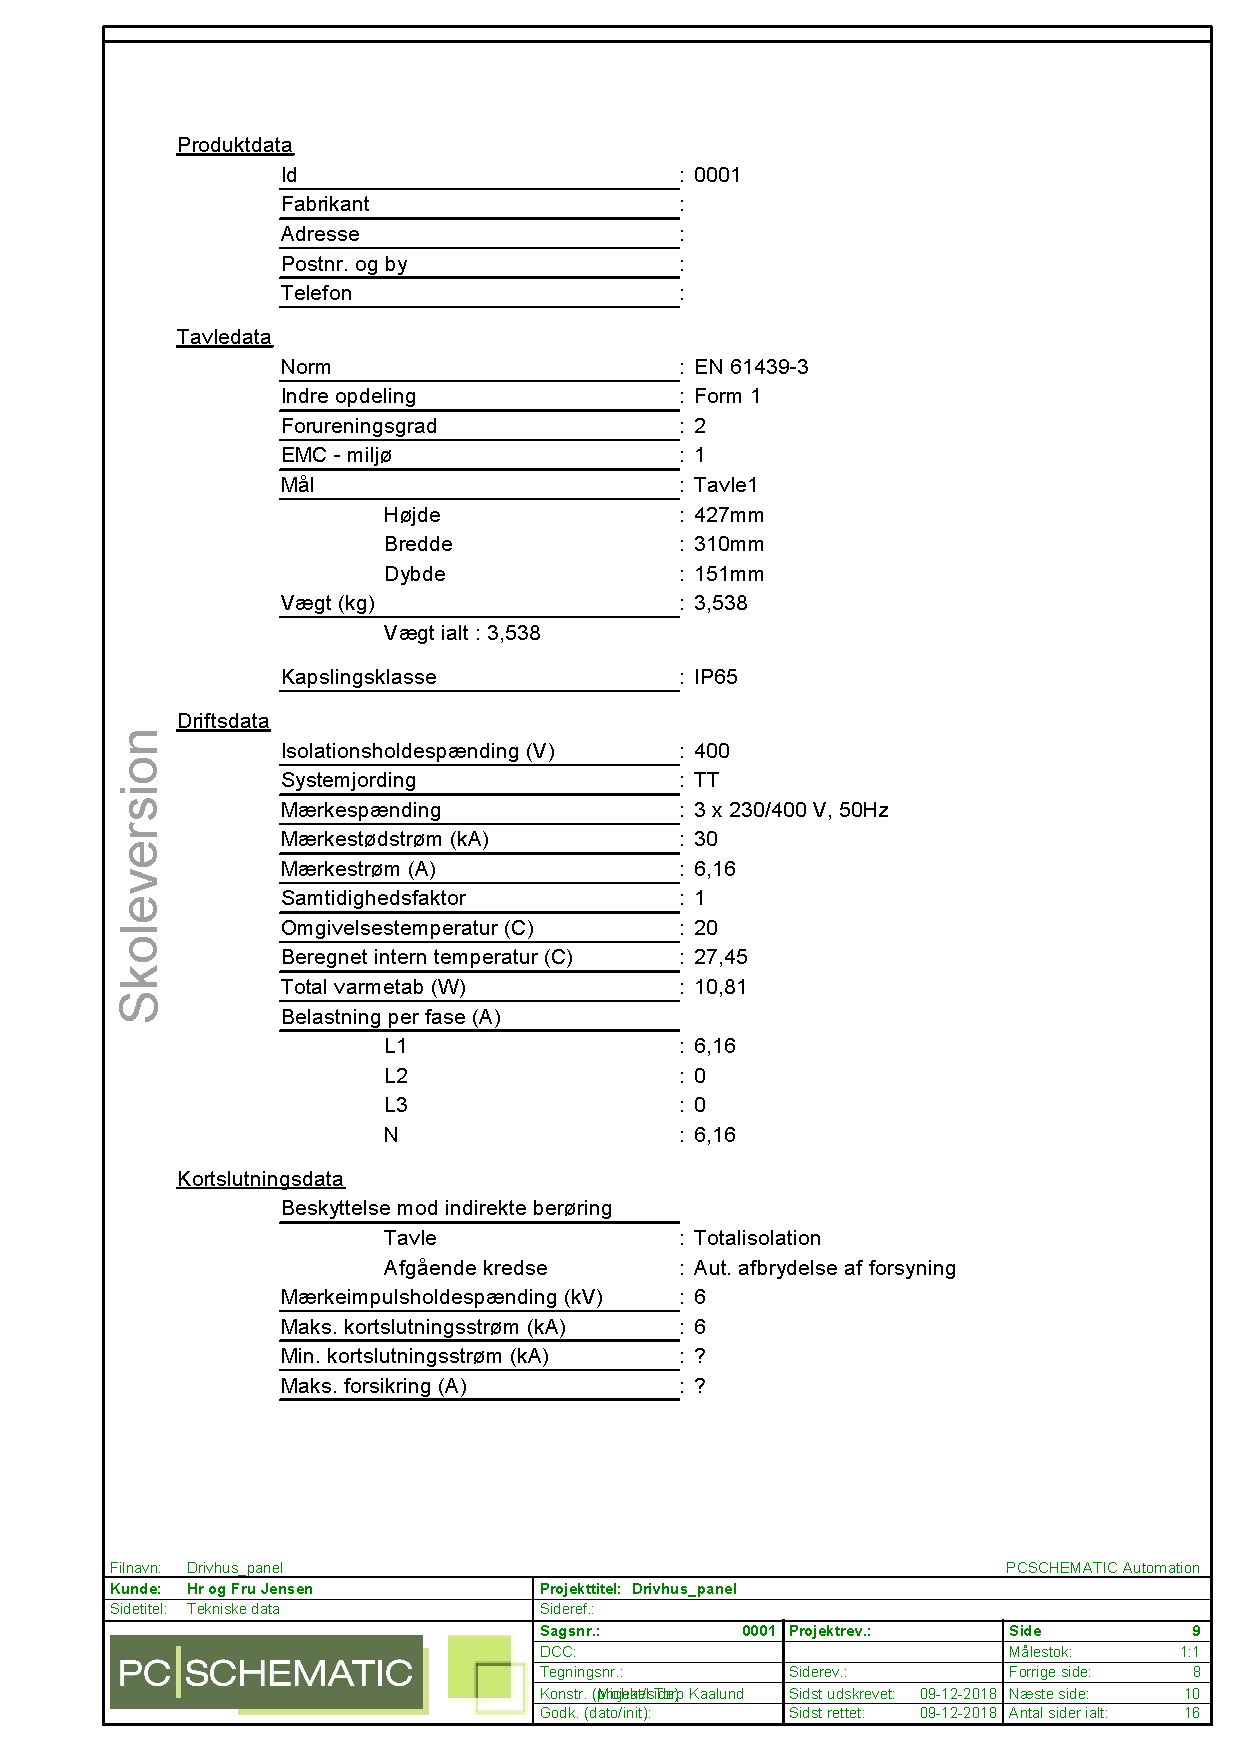
\includegraphics[scale=0.72]{appendix/Drivhus_panel_12.pdf}
\newpage
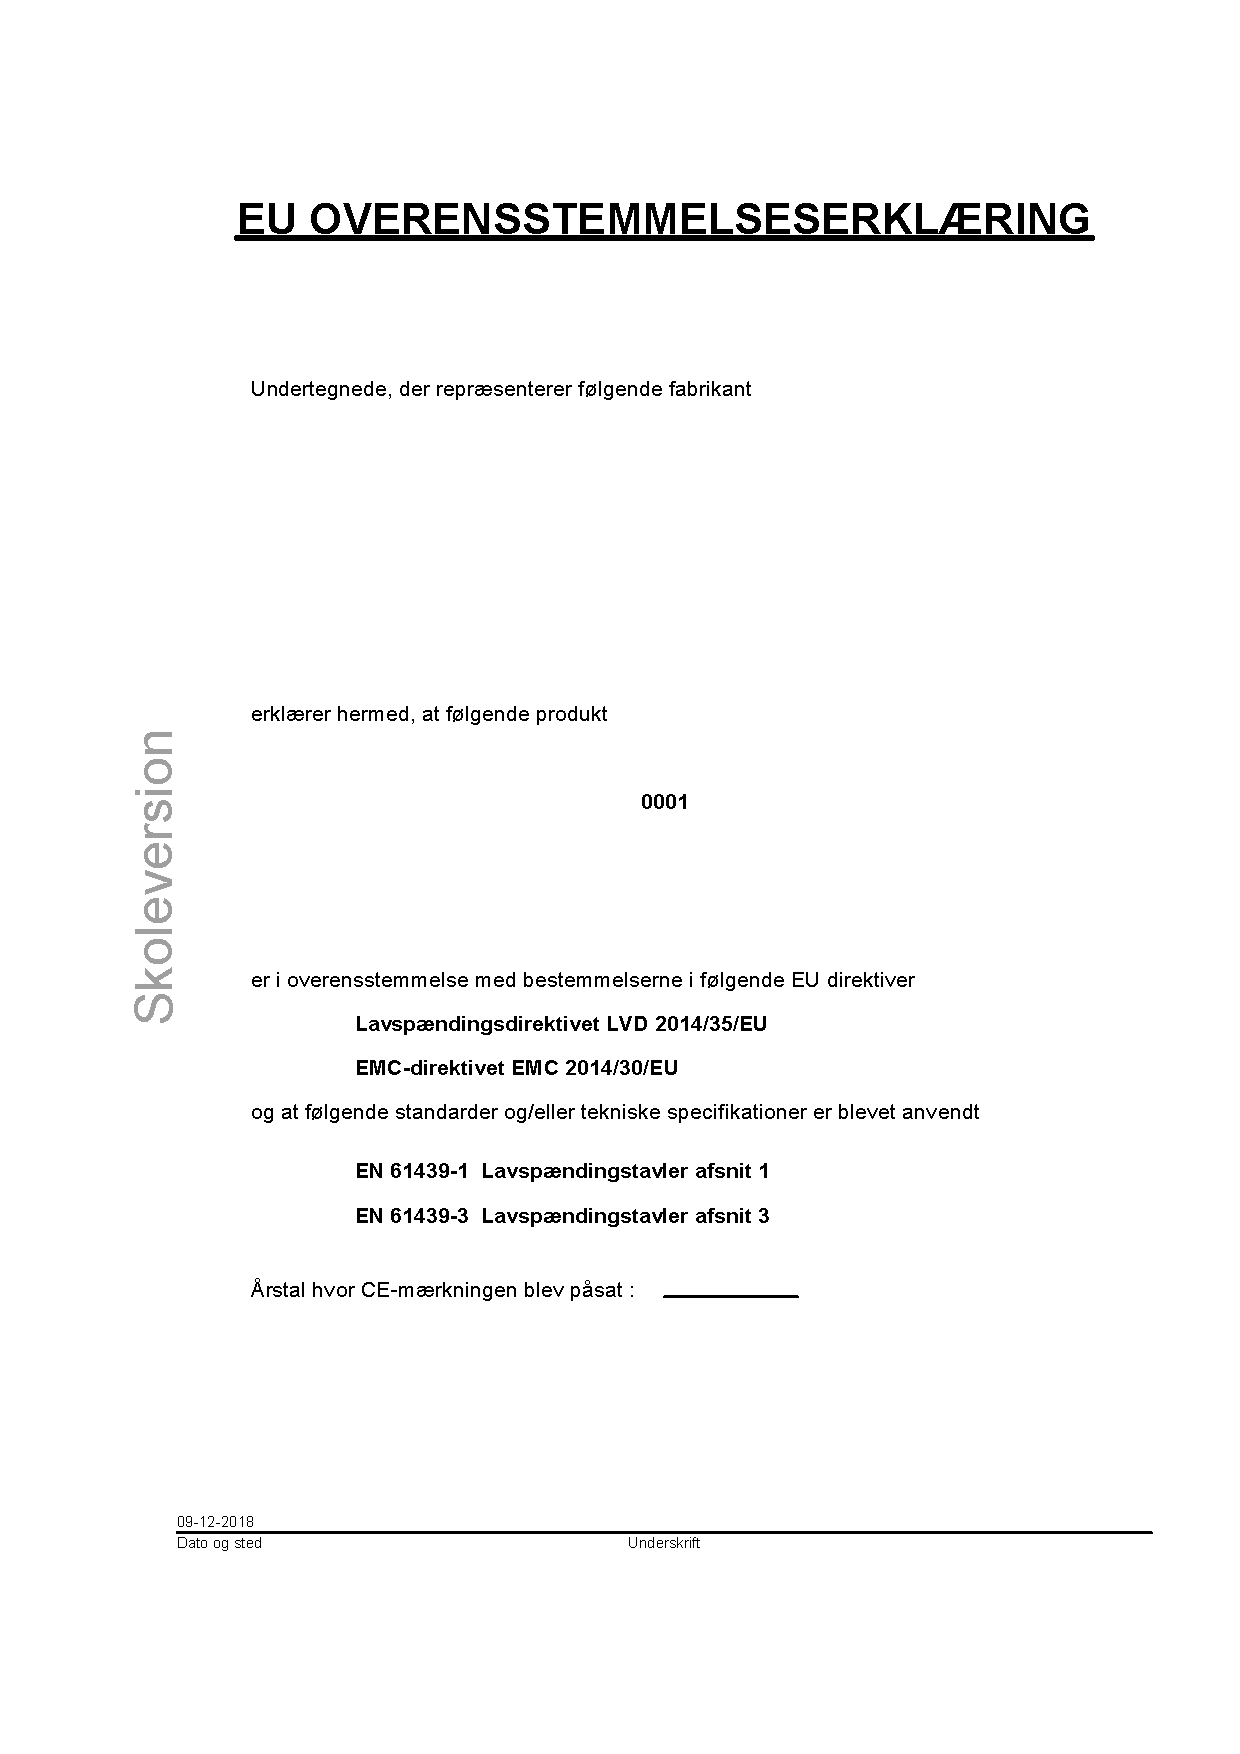
\includegraphics[scale=0.72]{appendix/Drivhus_panel_13.pdf}
%\section{Siemens LOGO! Software}
%\newpage 
%\begin{figure}[!htp]
    %\centering
\subsubsection{Funktionsblokke}
\includegraphics[scale=0.72,angle=90,origin=c]{../LOGO_Program/drivhus_styring_1.pdf}
%\end{figure}
%\newpage
%\begin{figure}[!htp]
    %\centering
\subsubsection{Parameter}
\includegraphics[scale=0.72]{../LOGO_Program/drivhus_styring_2.pdf}
%\end{figure}
\newpage
%\begin{figure}[!htp]
    %\centering
\includegraphics[scale=0.72]{../LOGO_Program/drivhus_styring_3.pdf}
%\end{figure}
%\newpage
%\begin{figure}[!htp]
    %\centering
%\subsection{Kabel forbindelse}
%\includegraphics[scale=0.78]{../LOGO_Program/drivhus_styring_4.pdf}
%\end{figure}
%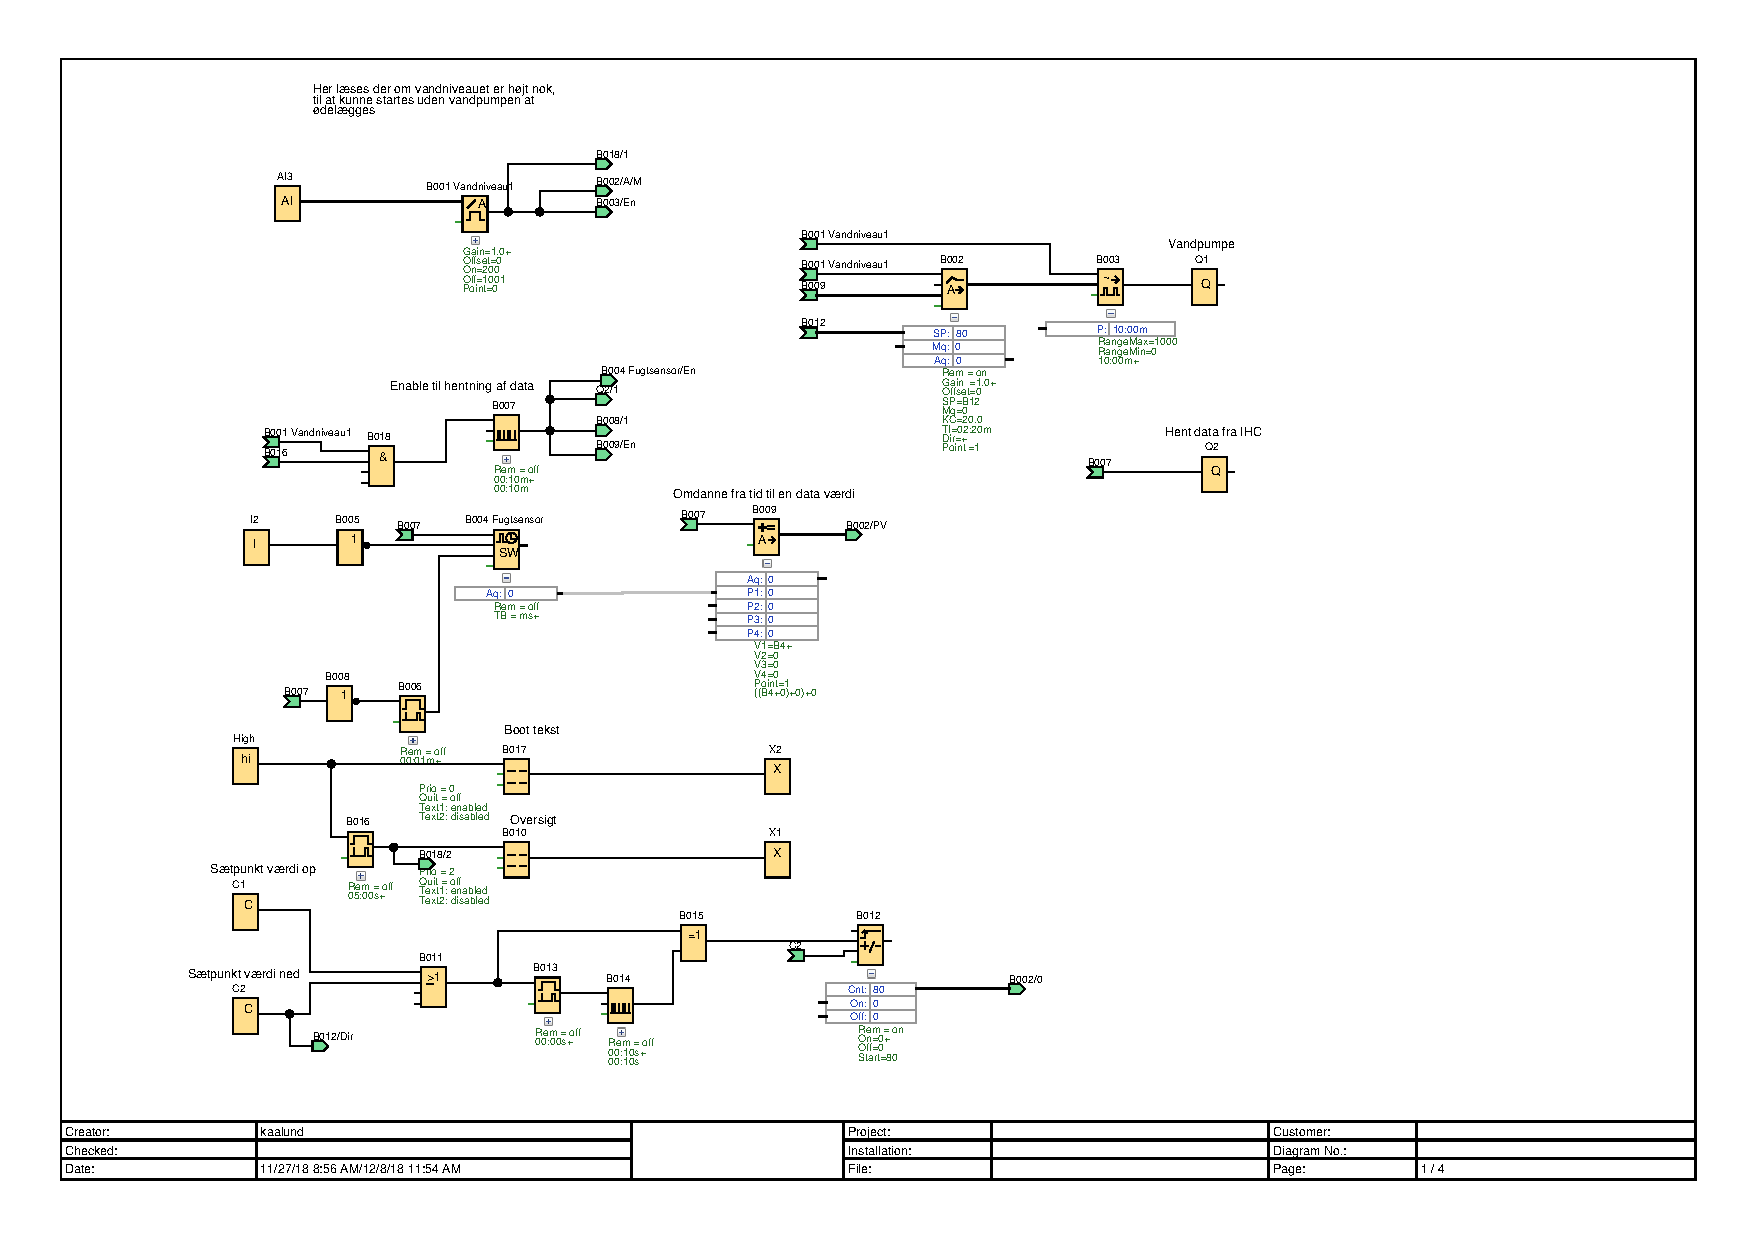
\includepdf[pages=-]{../LOGO_Program/Drivhus_program.pdf}
    \section{Home-Assistant}

\subsection{Installationen af Home-Assistant på Raspberry Pi 3 model B+}
Der er en god guide på \url{https://www.home-assistant.io/getting-started/} som anbefales, at følge.
Men den er dog på engelske. Jeg har valgt, at lave en kort beskrivelse af installationen på dansk.
\\
\\
Der er to måder, at installere home-assistant på den ene er at installere den på en eksisterende raspbian billedefil og den anden er at hente en forud konfigueret hass.io billedfil.
Jeg har dog kun valgt, at beskrive installationen af hass.io til Raspberry Pi 3 model B+, da den anden metode er for advanceret bruger af Raspberry Pi og linux styresystemet.


\subsection{Opsætning}
\subsection{Scener}

\end{document}